\documentclass[apjl]{emulateapj}

\usepackage{hyperref}
\usepackage{amsmath}
\usepackage{amssymb}
\usepackage{graphicx}
\usepackage{color}
\usepackage{natbib}

\newcommand{\MSun}{M_\odot}
\newcommand{\RSun}{R_\odot}
\newcommand{\Rstar}{R_*}
\newcommand{\Mstar}{m_*}
\newcommand{\MBH}{M_\mathrm{BH}}

\def\aj{Astronomical Journal}                 % Astronomical Journal
\def\apj{Astrophysical Journal}                % Astrophysical Journal
\def\apjl{Astrophysical Journal}             % Astrophysical Journal, Letters
\def\pasj{PASJ}
\def\apjs{ApJS}              % Astrophysical Journal, Supplement
\def\mnras{MNRAS}            % Monthly Notices of the RAS
\def\prd{Phys.~Rev.~D}       % Physical Review D
\def\prl{Phys.~Rev.~Lett}    % Physical Review Letters
\def\cqg{Class.~Quant.~Grav.~}%Classical and Quantum Gravity
\def\araa{ARA\&A}             % Annual Review of Astron and Astrophys
\def\nat{Nature}              % Nature
\def\aap{A\&A}                % Astronomy and Astrophysics
\def\na{New Astronomy}

\newcommand{\will}[1]{\textcolor{cyan}{#1}}
\newcommand{\ilya}[1]{\textcolor{red}{#1}}

\newcommand{\onesigrange}[3]{\ensuremath{#1^{+#2}_{-#3}}}
\newcommand{\alpharange}{\onesigrange{2.27}{0.17}{0.15}}
\newcommand{\alpharangeHM}{\onesigrange{2.55}{0.23}{0.21}}

\begin{document}

\title{Comment on ``An excess of massive stars in the local 30 Doradus starburst''}

\author{Will Farr\altaffilmark{1}, Ilya Mandel\altaffilmark{1}}
\affil{$^1$Institute of Gravitational Wave Astronomy and School of Physics and Astronomy, University of Birmingham, Birmingham, B15 2TT, United Kingdom}
\email{wmfarr@star.sr.bham.ac.uk, imandel@star.sr.bham.ac.uk}

\begin{abstract}
Schneider et al. (Reports, 5 January 2018, p.~69) found more massive stars in the 30 Doradus star-forming region above 30 solar masses than predicted by a standard Salpeter initial mass function (IMF).  Their finding of an IMF power-law exponent of $1.90^{+0.37}_{-0.26}$ is based on a flawed statistical analysis of the data.  We re-analyze their data with appropriate statistical tools to find an IMF exponent of $\alpharange$, consistent with the Salpeter value of $2.35$.
\end{abstract}

\maketitle

The universality of the initial mass function of stars is a hot topic in modern astrophysics, with impact on galactic evolution, supernovae, and gravitational-wave sources \cite{Kroupa:review,Bastian:2010}.    \citet{Schneider:2018} use spectroscopic observations of young massive stars in the 30 Doradus region of the Large Magellanic Cloud to infer a shallower-than-expected IMF.  Their conclusion is due to a faulty statistical methodology.  

\citet{Schneider:2018} obtain estimates of the ages and masses of individual stars with the BONNSAI Bayesian code \cite{Schneider:Bonn}.  They then obtain an overall mass distribution by effectively adding together the posterior probability density functions of individual stars.  There is no statistical meaning to a distribution obtained in this way, and it does not represent the posterior probability density function on the underlying mass distribution.  In fact, for a steeply decaying power law underlying distribution such as the one being considered here, the approach of \cite{Schneider:2018} will yield a distribution biased toward the high-mass end.  The measurement uncertainty will ``smear out'' the masses of both low-mass and high-mass stars, but because there are far more low-mass stars than high-mass ones, this appears to yield more mass at the high end of the distribution, leading to a false conclusion of a shallower distribution.

Hierarchical Bayesian inference provides the statistically correct solution to this problem \cite{Hogg:2010}.  \citet{Mandel:2010stat} specifically considered inference on a mass distribution given a sample of uncertain measurements, and we use this methodology here.  We follow \citet{Schneider:2018} in assuming that their data set is complete above 15 solar masses.  We interpret their inference on individual masses and ages as log-normal likelihoods with parameters fixed by matching the peak and 68\% width of the individual stellar distributions to the \citet{Schneider:2018} data.  We model the star formation history as a Gaussian distribution.  We use the Hamiltonian Monte Carlo sampler STAN \cite{STAN} to efficiently address the high-dimensional hierarchical problem with free parameters for each star's actual mass and birth age in addition to the IMF slope and the mean and standard deviation of the star formation history.

Figure \ref{fig:IMF} shows the inferred power-law exponent of the IMF.  We find
an exponent of $\alpharange$ where the quoted value corresponds to the peak of
the posterior distribution and the range to the 17th and 83rd percentiles.  The
conclusion is somewhat sensitive to the choice of the cutoff mass for survey
completeness, with an exponent of $\alpharangeHM$ for a cutoff at $20 M_\odot$
rather than $15 M_\odot$.  However, these fluctuations are within the expected
statistical variation based on the sample size, as confirmed with posterior
predictive checking.

\begin{figure}
%\vspace{-1in}
    		    		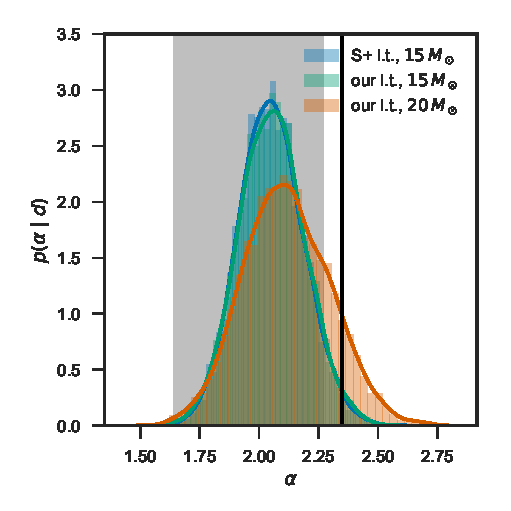
\includegraphics[trim={0cm 0cm 0cm 0cm},clip,scale=0.4]{alpha.pdf}
%\vspace{-1in}
    		\caption{Blah}\label{fig:IMF}
\end{figure}

We confirm the stability of our conclusions with posterior predictive checking.  Figure \ref{fig:PPC} shows the inferred mass distribution from the data on top of the range of mass distributions that would be inferred from a large number of data sets drawn according to our preferred IMF model.  The data can be seen to be consistent with our IMF model.

\begin{figure}
%\vspace{-1in}
    		    		\includegraphics[trim={0cm 0cm 0cm 0cm},clip,scale=0.4]{dNdm-ppc-band.pdf}
%\vspace{-1in}
    		\caption{Blah}\label{fig:PPC}
\end{figure}


In conclusion, we find that there is no evidence for a deviation from the Salpeter IMF in the observations of young massive stars in 30 Doradus once correct statistical analysis is applied.

\bibliographystyle{hapj}
\bibliography{Mandel}
\end{document}
